% =====================================================================
% Full assembled Error Analysis section (paste-ready).
% Replaces the current \subsection{Error analysis} in main.tex.
% Order: kept intro paragraph -> A0 (FP/FN) -> kept error_map figure
%        -> A (four constraints + table) -> B (diagnostics figure)
%        -> C (claim + future work).
% New figure to include: figs/constraint_diagnostics.pdf
% =====================================================================

\subsection{Error analysis}\label{sec:error-analysis}

% --- KEPT: opening decomposition paragraph ---
\hl{To understand why the absolute metrics remain limited, we decomposed each predicted point into four outcomes against the ground truth: correct, false negative (FN, a block point labelled as background), false positive (FP, a background point labelled as a block), and class swap (a block point assigned to the wrong block type). The three error outcomes correspond to three failure modes. When the ring or block masks are not recovered, block points collapse into the background and errors appear as false negatives (under-segmentation). When background or non-lining points are absorbed into a block mask, errors appear as false positives (over-segmentation); these remain rare in practice. When the geometric boundaries are detected but the positional block labels are shifted, errors appear as class swaps. The remaining errors therefore do not indicate one uniform failure of R4Tun; they show where the fixed SAM4Tun substrate is still sensitive to geometry, density, and labelling assumptions.}

% --- BLOCK A0: FP/FN composition paragraph + table ---
\hl{Quantifying this decomposition over all ground-truth points (Table~\ref{tab:error-composition}) shows that the two categories carry different failure modes, and that adaptation acts on them differently. On regular tunnels, the baseline error is split between missed blocks (false negatives, $21\%$) and wrong block classes (class swaps, $26\%$); \mbox{$m+s+k$} almost eliminates the false negatives ($21\%\rightarrow2\%$) but the class swaps persist ($26\%\rightarrow21\%$). On complex tunnels, the baseline is almost entirely under-segmentation: $66\%$ of points are false negatives and essentially none are class swaps, because the blocks are not recovered at all. Adaptation recovers most of these blocks ($66\%\rightarrow17\%$ false negatives), but the recovered points are then mislabelled rather than corrected, so class swaps rise from $0\%$ to $34\%$. False positives stay small throughout ($\leq6\%$). The residual error is therefore a labelling problem (class swap), not a detection or noise problem (false positive), which points directly at the positional labelling rule analysed below.}

\begin{table}[ht]
\caption{\hl{Error composition as a fraction of ground-truth points (Opus-4.6 \mbox{$m+s+k$} vs.\ SAM4Tun baseline; Regular $n=13$, Complex $n=17$). FN: block predicted as background; FP: background predicted as block; swap: block predicted as the wrong block class. Adaptation removes false negatives; the residual error is dominated by class swaps.}}\label{tab:error-composition}
\begin{tabular*}{\tblwidth}{@{} l l c c c c @{}}
\toprule
Category & Method & Correct & FN & FP & Swap \\
\midrule
\multirow{2}{*}{Regular}
  & SAM4Tun     & 51\% & 21\% & 3\% & 26\% \\
  & \mbox{$m+s+k$} & 71\% & 2\%  & 5\% & 21\% \\
\midrule
\multirow{2}{*}{Complex}
  & SAM4Tun     & 34\% & 66\% & 0\% & 0\%  \\
  & \mbox{$m+s+k$} & 43\% & 17\% & 6\% & 34\% \\
\bottomrule
\end{tabular*}
\end{table}

% --- KEPT: error_map figure (Fig. 11) ---
\begin{figure*}[t]
\centering
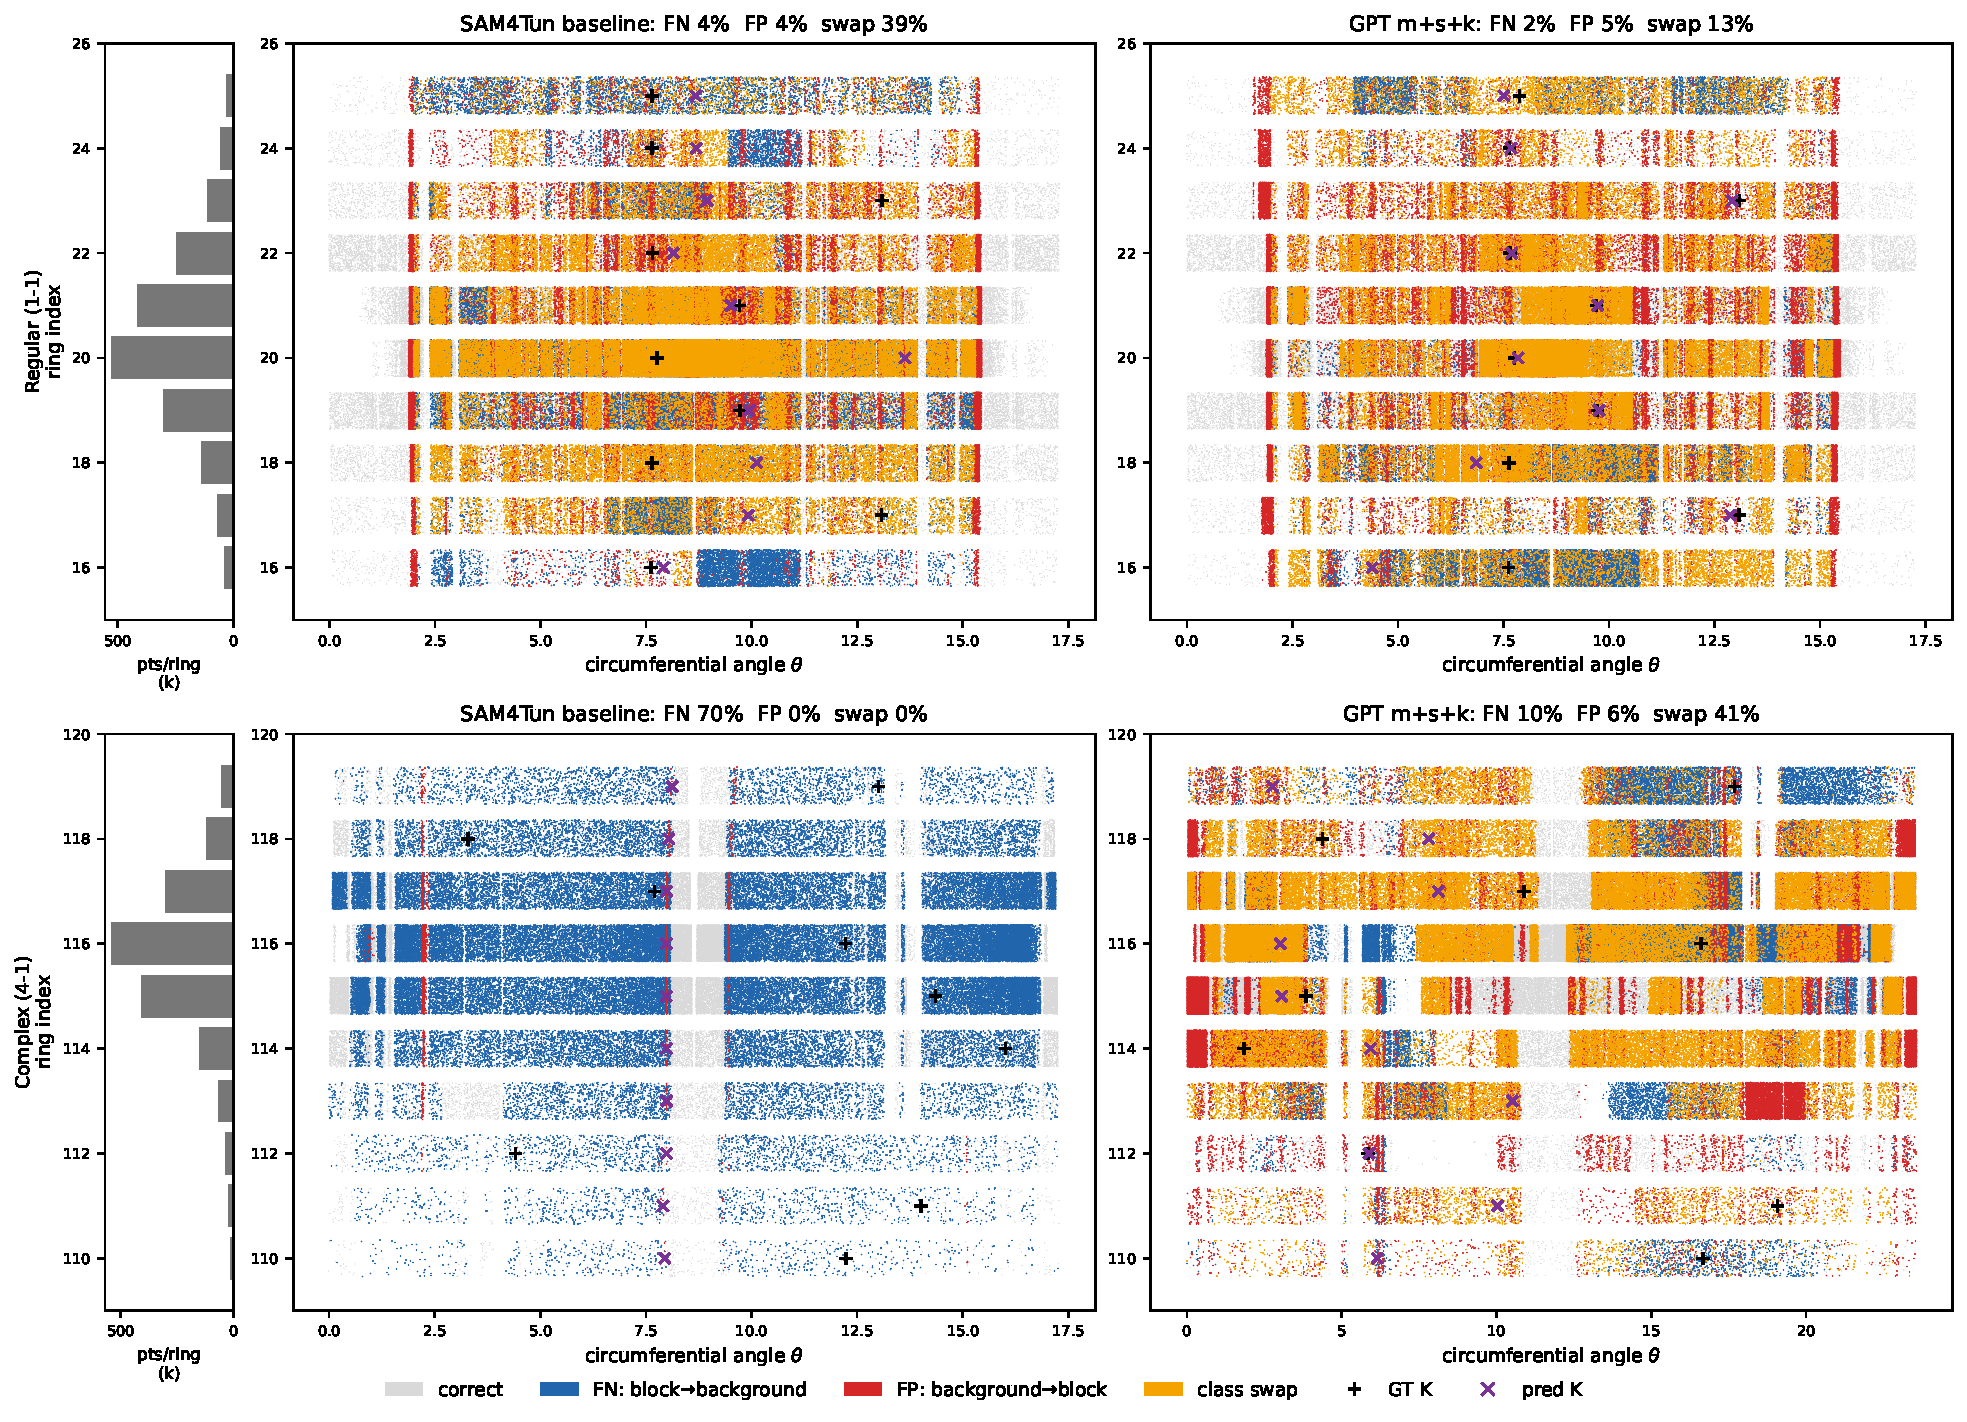
\includegraphics[width=\textwidth]{figs/error_map.pdf}
\caption{\hl{FP/FN error map drawn as a ring-by-\mbox{$\theta$} raster. Each row is one ring, \mbox{$\theta$} is the circumferential angle, and each point is coloured as correct, false negative, false positive, or class swap. The examples illustrate the two regimes: on regular tunnels such as tunnel 1-1, boundaries are often present but labels can rotate into neighbouring block classes, producing class swaps (23\% of evaluated points, with FN and FP each about 2\%); on complex tunnels such as tunnel 4-1, under-segmentation dominates and many block points are labelled as background (69\% FN). The map is intended to localise the remaining errors rather than to introduce a new performance metric.}}
\label{fig:error-map}
\end{figure*}

% --- BLOCK A: four structural constraints + quantification table ---
\hl{Both failure modes trace back to the positional labelling rule in the fixed SAM4Tun substrate: each ring is labelled by first detecting the key block (K), then placing the remaining blocks by stepping through a fixed angular template above and below K. This rule is efficient and auditable, and it is exactly the part of the pipeline that R4Tun does not re-parameterise. It also creates four structural constraints, which we quantify across the 30 tunnels in Table~\ref{tab:error-constraints} (Opus-4.6 \mbox{$m+s+k$} versus the SAM4Tun baseline; accuracy denotes ground-truth block-class accuracy).}

\begin{enumerate}
\item \hl{\emph{Non-uniform point density.} Central rings are far denser than end rings: within a single tunnel the per-ring point count varies by up to $19\times$ (regular) and $38\times$ (complex). A single tunnel-level preprocessing setup cannot match this range, and per-ring density correlates positively with accuracy ($+0.34$ on regular), so sparse rings systematically lose ring-boundary and K-anchor detection.}
\item \hl{\emph{Moving K-anchor.} Staggered and interleaved assembly shifts K along the arc from ring to ring. The fraction of K-mislocated rings rises from $12\%$ (regular) to $64\%$ (complex); once K is misidentified the whole ring's labels rotate together, and accuracy collapses from $0.64$ to $0.24$ (regular) and from $0.28$ to $0.14$ (complex). This is the dominant limiter on complex tunnels.}
\item \hl{\emph{Fixed segment-offset template.} Each block is placed at a fixed angular offset from K. Where the $6$-segment template matches the geometry (regular), recall is near-uniform with distance from K; where it does not (the $7$-segment complex tunnels), the mismatch appears from the first offset and the block adjacent to K drops to $0.23$ recall even on rings where K is correctly located.}
\item \hl{\emph{Hard-coded walk direction.} B- and A-blocks are walked from K on a fixed side. When a ring's physical handedness is reversed, the predicted labels become a mirror image of the ground truth: this occurs on $17/130$ regular and $28/166$ complex rings (concentrated in continuous and reversed-handedness tunnels), where accuracy falls to about $0.08$. A mirror flip cannot be corrected by parameter tuning.}
\end{enumerate}

\begin{table*}[t]
\caption{\hl{Quantified structural constraints of the fixed SAM4Tun positional-labelling rule (Opus-4.6 \mbox{$m+s+k$}, $n=30$; Regular $n=13$, Complex $n=17$). Values are computed from ground-truth versus predicted block labels; ``accuracy'' is ground-truth block-class accuracy. These quantities are properties of the labelling rule, not parameter values, so bounded adaptation can approach but not remove the resulting ceiling.}}\label{tab:error-constraints}
\begin{tabular*}{\textwidth}{@{\extracolsep{\fill}} l l l l l @{}}
\toprule
Constraint & What we quantify & Regular & Complex & Effect on accuracy \\
\midrule
C1: Non-uniform density &
\parbox[t]{0.24\textwidth}{\raggedright per-ring count max/min; corr(density, accuracy)} &
$19\times$; $+0.34$ & $38\times$; $+0.10$ &
\parbox[t]{0.24\textwidth}{\raggedright sparse end rings lose boundaries; one config cannot span the range} \\
\midrule
C2: Moving K-anchor &
\parbox[t]{0.24\textwidth}{\raggedright K-mislocated rings; accuracy aligned vs.\ mislocated} &
$12\%$; $0.64{\to}0.24$ & $64\%$; $0.28{\to}0.14$ &
\parbox[t]{0.24\textwidth}{\raggedright mislocated K rotates the whole ring; dominant complex limiter} \\
\midrule
C3: Fixed segment-offset template &
\parbox[t]{0.24\textwidth}{\raggedright recall near-K vs.\ far-K (K-aligned rings)} &
$0.66$--$0.69$ (uniform) & $0.23$ at first offset &
\parbox[t]{0.24\textwidth}{\raggedright 6-step template fits regular; mismatches 7-segment complex} \\
\midrule
C4: Hard-coded walk direction &
\parbox[t]{0.24\textwidth}{\raggedright mirror-flip rings (of total); flip-ring accuracy} &
$17/130$; $\approx0.08$ & $28/166$; $\approx0.10$ &
\parbox[t]{0.24\textwidth}{\raggedright reversed handedness mirror-images labels; not tunable} \\
\bottomrule
\end{tabular*}
\end{table*}

% --- BLOCK B: diagnostics figure (replaces error_mechanism.pdf) ---
\begin{figure*}[t]
\centering
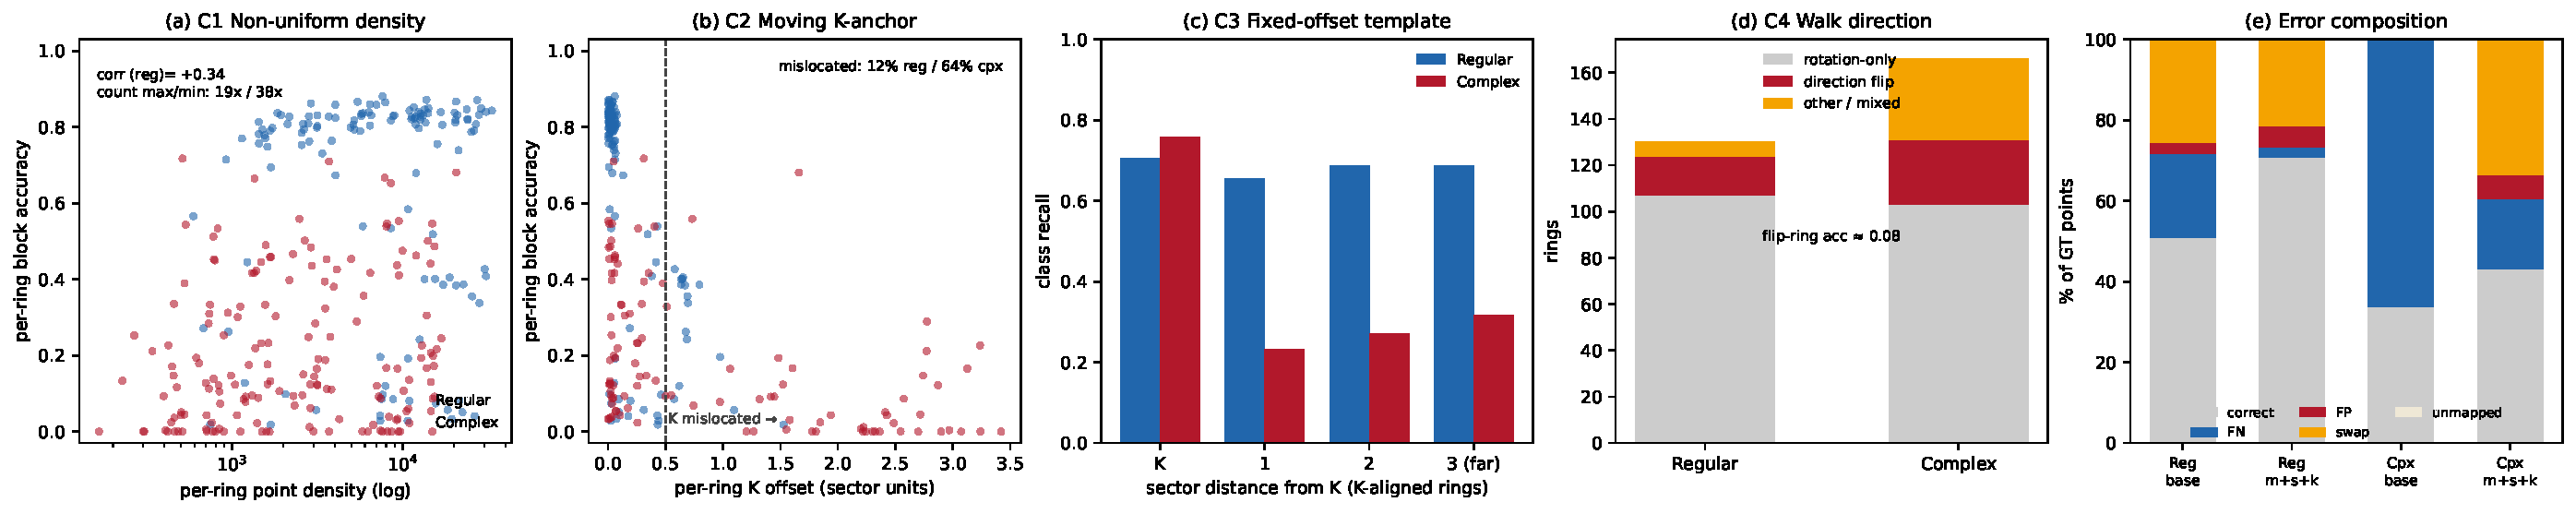
\includegraphics[width=\textwidth]{figs/constraint_diagnostics.pdf}
\caption{\hl{Quantitative diagnostics for the four structural constraints (Opus-4.6 \mbox{$m+s+k$}, 30 tunnels). (a)~C1: per-ring point density versus per-ring block accuracy; sparse rings (left) segment poorly and complex rings (red) cluster low. (b)~C2: per-ring K offset (in sector units) versus accuracy; beyond half a sector the K-anchor is mislocated and accuracy collapses, far more often on complex tunnels. (c)~C3: class recall by sector distance from K on K-aligned rings; the fixed 6-step template is near-uniform on regular tunnels but fails at the first offset on 7-segment complex tunnels. (d)~C4: per-ring ordering outcomes; most rings are pure rotations, but hard-coded walk direction yields mirror flips whose accuracy is about 0.08. (e)~error composition as a fraction of ground-truth points (baseline vs.\ \mbox{$m+s+k$}, by category): adaptation removes false negatives (under-segmentation) while the residual error is dominated by class swaps from the labelling rule, with false positives staying small. The panels localise and size the remaining errors; they do not introduce a new performance metric.}}
\label{fig:error-mechanism}
\end{figure*}

% --- BLOCK C: rewritten claim + future-work paragraph ---
\hl{This analysis clarifies the claim supported by the experiments and is consistent with how we position R4Tun in Section~\ref{sec:intro}. R4Tun adapts the parameter-sensitive parts of the fixed pipeline, especially Hough thresholds, mask radii, padding, and interpolation settings, and these adaptations recover a large share of the achievable accuracy (regular block accuracy $0.35\to0.67$; complex $0.00\to0.23$). They do not, however, change the positional labelling rule, and Table~\ref{tab:error-constraints} shows that the residual error is governed by that rule rather than by a failure of LLM reasoning: K-mislocation and the fixed template, not parameter choices, set the complex-tunnel ceiling. We therefore read the low complex-tunnel mIoU as a property of the single-reference SAM4Tun substrate, and we report these constraints openly because they define the configuration challenge that bounded adaptation is asked to address.}

\hl{Removing these constraints is future work rather than a parameter change, because each is built into the detect-K-then-fixed-template labelling logic of SAM4Tun. Density-adaptive preprocessing, per-ring K re-anchoring, a variable-length segment template, and handedness inference would replace that logic with dynamic, context-aware labelling; in the current open-source implementation this requires re-writing the labelling stage, which lies outside the bounded-parameter adaptation studied here. Encoding multiple expert reference configurations (Section~\ref{sec:limitations}) would also raise the ceiling. These directions extend, and do not invalidate, SAM4Tun or R4Tun: the present study establishes that structured context lets an LLM adapt parameters within fixed bounds, and isolates exactly which structural parts of the substrate must change next to lift the absolute ceiling.}
